% Name: Cost curves
% Description: A firm's marginal, average total, and average variable cost, with marginal cost crossing each average at its lowest point.
% Tags: cost curves, marginal cost, average cost, firm theory

\usepackage{pgfplots}
\pgfplotsset{compat=1.18}

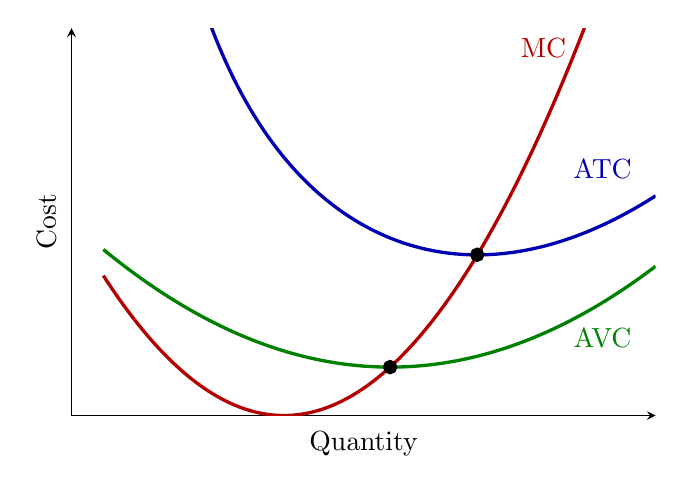
\begin{tikzpicture}
  % Total cost 16 + 4q - q^2 + q^3/12: AVC is lowest at q = 6, ATC near q = 7.64, and MC passes through both.
  \begin{axis}[
    width=9cm, height=6.5cm, xmin=0, xmax=11, ymin=0, ymax=8,
    axis lines=left, xlabel=Quantity, ylabel=Cost,
    xtick=\empty, ytick=\empty, domain=0.6:11, samples=120,
    every axis plot/.append style={very thick},
    clip=true,
  ]
    \addplot[red!70!black, domain=0.6:9.66] {4 - 2*x + x^2/4};
    \addplot[blue!70!black, domain=2:11] {16/x + 4 - x + x^2/12};
    \addplot[green!50!black] {4 - x + x^2/12};
    \node[red!70!black, left] at (axis cs:9.5,7.6) {MC};
    \node[blue!70!black, above] at (axis cs:10,4.7) {ATC};
    \node[green!50!black, below] at (axis cs:10,2) {AVC};
    \addplot[only marks, mark=*, mark size=2pt] coordinates {(6,1) (7.64,3.32)};
  \end{axis}
\end{tikzpicture}
